\documentclass{beamer}

\graphicspath{{../Images/}} % the folder in which images are stored for this project
\usepackage{tikz,graphicx,amsmath,hyperref,tcolorbox,fancyvrb,xcolor}
\hypersetup{colorlinks=true} % make sure our hyperlinks are coloured for visibility
\definecolor{DBlack}{RGB}{35,31,32}
\definecolor{DPurple}{RGB}{126,49,123}
\definecolor{DBlue}{RGB}{0,99,136}

\tcbuselibrary{skins,breakable}
\newenvironment{BGVerbatim}
 {\VerbatimEnvironment
  \begin{tcolorbox}[
    breakable,
    colback=lightgray,
	boxsep=3mm
  ]%
  \begin{Verbatim}}
 {\end{Verbatim}\end{tcolorbox}}

\usecolortheme[RGB={83,13,88}]{structure}
% This is the theme that we are modifying
\usetheme{Boadilla}

% Change the font colour to white on the title page to stand out against the purple
\setbeamercolor{title}{fg=white}
\setbeamerfont{title}{family=\rmfamily}
\setbeamercolor{author}{fg=white}
\setbeamerfont{author}{series=\bfseries}
\setbeamercolor{institute}{fg=white}
\setbeamercolor{date}{fg=white}
\setbeamerfont{date}{series=\bfseries}

% Remove the default ball bullet points in the toc, but keep the numbering
\setbeamertemplate{sections/subsections in toc}[sections numbered]
% Change the item icons to be circles rather than balls
\setbeamertemplate{itemize items}[circle]
% Define blocks to be rounded rectangles with shadows
\setbeamertemplate{blocks}[rounded][shadow=true]

% Turn the @ symbol into character class other
\makeatother
% Modify the footline to get a two part footline with slide numbers
\setbeamertemplate{footline}
{
  \leavevmode%
  \hbox{%
  % Create a box with width of slide, containing current slide and total slides
  \begin{beamercolorbox}[wd=\paperwidth,ht=2.25ex,dp=1ex,center]{section in head/foot}%
    \insertframenumber{} / \inserttotalframenumber\hspace*{1ex}
  \end{beamercolorbox}}%
  \vskip0pt%
}
% Turn the @ symbol back to a letter
\makeatletter

% Remove the default navigation symbols from the bottom of the slides
\setbeamertemplate{navigation symbols}{}

\author{Sam Fearn}
%\institute[Durham]{Durham University}
\title{A Very Quick Introduction To \LaTeX{}}
\date{March 15\textsuperscript{th}, 2019}

\begin{document}
    
% --- Start Custom Commands --- %

% --- End Custom Commands --- %

%--- the titlepage frame -------------------------%
{
% Draw a purple box for the background of the title slide and add the durham logo at the bottom
\setbeamertemplate{background canvas}{
\begin{tikzpicture}
    \clip (0,0) rectangle (\paperwidth,\paperheight);
    \fill[color=DPurple] (0,0) rectangle (\paperwidth,\paperheight);
    \node[inner sep=0pt] (MathsLogo) at (1.5,8.3)
        {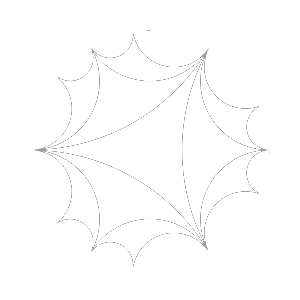
\includegraphics[width=20mm]{MathsLogo.png}};
\end{tikzpicture}
}

\begin{frame}[plain]
\maketitle
\end{frame}
}

%---Complete Outline--------------------%
\begin{frame}
       \frametitle{Outline}
       \tableofcontents
\end{frame}
% (end)

\section{What is \LaTeX{}?}
\label{sec:introduction}
\begin{frame}{What is \LaTeX{}?}
	\begin{itemize}
		\item<1-> \LaTeX{} (built on \TeX{}) is a system for producing formatted text-based documents.
		\item <2-> Unlike a word processor (such as Microsoft Word), the document is written in plain text, without formatting.
		\item <3-> Markup commands are included in order to tell \LaTeX{} how the document should look.
		\item <4-> \LaTeX{} makes many decisions automatically in order to easily produce high quality (usually PDF) output that doesn't require the reader to own proprietary software.
		\item <5-> \LaTeX{} is open source and free!
		\item <6-> \LaTeX{} was designed to make typesetting mathematical formulae easy.
	\end{itemize}
\end{frame}
%--- Next Frame ---%

\section{How Do I Use \LaTeX{}?}
\label{sec:how_do_i_use_latex}
\begin{frame}{How Do I Use \LaTeX{}}
	Since a \LaTeX{} (\TeX{}) document is written in plain text, any plain text editor (Notepad, TextEdit, Gedit, Leafpad, Vim $\ldots$) can be used to write the tex file.
	
	\pause
	\medskip
	
	However, in order to produce the formatted output, the tex file must be `typeset' using the \LaTeX{} system to produce a PDF of your document.
	
	\pause
	\medskip
	
	On the computers in university computing rooms we can run \LaTeX{} by launching `Latex - Miktex' from the App hub, then launching TeXWorks from the start menu, under MiKTeX. You can also use TeXStudio.
	
	\pause
	\medskip
	
	\LaTeX{} is free software and can be easily installed on your own computers. The department recommends Windows users install \href{http://miktex.org/}{MiKTeX (miktex.org)} and macOS/OS X users install \href{http://www.tug.org/mactex/}{MacTeX (http://www.tug.org/mactex/)}. These come with specialised \LaTeX{} frontends (editors).
	
	\pause
	\medskip
	
	There exist mobile apps capable of producing \LaTeX{} documents, and you can also produce \LaTeX{} documents using a web browser with \href{https://www.overleaf.com}{Overleaf} (and others).
	
\end{frame}
%--- Next Frame ---%

\begin{frame}[fragile]{What Does A \LaTeX{} File Look Like?}
	Let's now look at the most basic example of a \LaTeX{} file:
	
\begin{BGVerbatim}[numbers=left,numbersep=10pt]
\documentclass{article}
\begin{document}
Some text here
\end{document}
\end{BGVerbatim}

\pause\medskip

Although this produces a document, it has very minimal formatting and isn't very attractive. Let's consider an example with some more structure.
\end{frame}

\begin{frame}[fragile]
\begin{BGVerbatim}[numbers=left,numbersep=10pt]
\documentclass{article}

% We define an Author, Title and Date
\author{Sam Fearn}
\title{A Very Quick Introduction To \LaTeX{}}
\date{March 15\textsuperscript{th}, 2019}

\begin{document}
% Create a title from our Author, Title and Date
\maketitle
\section{Introduction}
Some introductory text goes here
\section{Content}
The main content goes here
\end{document}
\end{BGVerbatim}

With very little effort we have a nicely formatted document.

\end{frame}

\section{Typesetting Mathematics In \LaTeX{}}
\label{sec:typesetting_mathematics_in_latex}
\begin{frame}[fragile]{Typesetting Mathematics In \LaTeX{}}
	\LaTeX{} is very good at typesetting mathematical formulae:
	
\begin{BGVerbatim}
If $\phi(x) = \frac{1}{\sqrt{2\pi}}e^{- x^2/2}$, then
\begin{equation}
	\Phi(x) := \int_{-\infty}^x \phi(t) dt.
\end{equation}
Moreover,
\begin{equation}
	\int_{-\infty}^\infty \frac{1}{\sigma
\sqrt{2\pi}} e^{-\frac{1}{2}\left(\frac{x-\mu}{\sigma}
\right)^2} dt = 1
\end{equation}
\end{BGVerbatim}

If $\phi(x) = \frac{1}{2\pi}e^{- x^2/2}$, then $\Phi(x) := \int_{-\infty}^x \phi(t) dt$. Moreover,
\begin{equation}
	\int_{-\infty}^\infty \frac{1}{\sigma\sqrt{2\pi}}e^{-\frac{1}{2}\left(\frac{x-\mu}{\sigma}\right)^2} dt = 1.
\end{equation}

\end{frame}

\begin{frame}[fragile]
Another example:

\begin{BGVerbatim}
We say a map $\psi:A \to B$ is \emph{injective} if
\begin{equation}
	\psi(a_1) = \psi(a_2) \implies a_1 = a_2,\ 
\forall\ a_1,a_2 \in A.
\end{equation}
\end{BGVerbatim}

We say a map $\psi:A \to B$ is \emph{injective} if
\begin{equation}
	\psi(a_1) = \psi(a_2) \implies a_1 = a_2,\ \forall\ a_1,a_2 \in A.
\end{equation}
\end{frame}

\section{Learning \LaTeX{}}
\label{sec:learning_latex}
\begin{frame}{Learning \LaTeX{}}
	The best way to learn \LaTeX{} is simply to start practicing using it. That's what the rest of this session is for.
	
	\medskip\pause
	
	Some useful resources to be aware of are:
	\begin{itemize}
		\item <2-> The department's page on \href{https://www.dur.ac.uk/mathematical.sciences/teaching/latex/}{\LaTeX{} for undergraduates}. This contains links to the relevant installers, as well as instructions for running \LaTeX{} on university computers.
		\item <3-> \href{https://tobi.oetiker.ch/lshort/lshort.pdf}{The Not So Short Introduction to \LaTeXe{}}, which contains almost everything you'll need to know about \LaTeX{} (for a while at least).
		\item <4-> \href{http://detexify.kirelabs.org/classify.html}{Detexify}, which lets you search for anything you can draw.
		\item <5-> \href{https://tex.stackexchange.com}{StackExchange} and \href{http://www.google.com}{Google}, where you'll find someone has almost certainly answered the question you have already.
		\item <5-> The help pages at \href{https://www.overleaf.com/learn}{Overleaf}.
	\end{itemize}
	
	\onslide<6->{You don't have to learn everything about \LaTeX{} initially, just start trying to write in \LaTeX{} and you'll figure it out as you go!}
	
\end{frame}

\section*{Thanks}
\begin{frame}[plain]
\begin{center}

\Huge
\only<1>{Questions?}
\end{center}

\only<2->{\Huge Activities:
\medskip
\normalsize
\begin{itemize}
	\item Try to reproduce the worksheet as closely as possible.
	\item Type up some of your discrete report in \LaTeX{}.
	\item Explore and modify the tex file for this talk. 
\end{itemize}}

\end{frame}

\end{document}